\section{Methodology}

In this section, we first formalize the problem setting and introduce the multi-agent modular design of \ours{}. We then detail the RL training recipe designed specifically for training the skill curator.

\subsection{Streaming Skill Curation with Multi-Agent Modular Design}

We consider a \textit{streaming} test-time setting~\citep{wu2024streambench}, where an LLM-based agent is deployed to solve a sequence of tasks
$\mathcal{D}=\{x_1,x_2,\dots,x_T\}$ that arrive over time. 
At each time stamp $t$, the agent must solve the current task $x_t$ before observing future tasks, producing an execution trajectory
$\xi_t=\{o_1,a_1,\dots,o_n,a_n\}$, where $o$ and $a$ denote observations and actions, respectively.
This setting naturally captures the challenge of self-evolving agents, where the system must distill useful experience from the trajectories of past interactions to improve performance on future tasks, and become more capable over time. Figure~\ref{fig: skillos_overview}\textcolor{redlinkcolor}{(a)} presents an overview of the system.

\noindent\textbf{Skill Repository.}
We maintain an external skill repository $\mathcal{S}_t$ at time stamp $t$, which consists of $N_t$ reusable skills
$\mathcal{S}_t=\{s_t^{1},s_t^{2},\dots,s_t^{N_t}\}$.
Following the widely adopted \texttt{SKILL.md} format~\citep{anthropic_skills_2025}, each skill is represented as a single Markdown file with two components as shown in Figure~\ref{fig: skillos_overview}\textcolor{redlinkcolor}{(b)}: 
(i) \textit{YAML frontmatter}, which specifies the skill name and a natural-language description of when the skill should be used, and 
(ii) \textit{Markdown instructions}, which describe the executable knowledge, workflows, constraints, and reusable heuristics captured by the skill.

\noindent\textbf{Agent Executor.}
Given a task $x_t$, a frozen agent executor $\pi_{\mathcal{L}}$ solves the task conditioning on the current environment observation and relevant skills.
Specifically, we retrieve a subset of skills $\tilde{\mathcal{S}}_{t}\subseteq \mathcal{S}_{t}$ using BM25~\citep{robertson2009probabilistic} for each task $x_t$, and the executor samples actions following
$a \sim \pi_{\mathcal{L}}(\cdot \mid x_t, o_t, \tilde{\mathcal{S}}_{t})$.

\noindent\textbf{Skill Curator.}
After the executor completes task $x_t$, the skill curator $\pi_{\mathcal{S}}$ observes the trajectory $\xi_t$, the self-judged correctness of the answers/interactions $\mathbbm{1}_{\xi_t}$, and a retrieved subset of related skills $\tilde{\mathcal{S}}_{t}$.
It then generates a sequence of structured curation operations
$c_t = (u_t^1,\dots,u_t^{M_t})
    \sim \pi_{\mathcal{S}}(\cdot \mid \xi_t, \mathbbm{1}_{\xi_t}, \tilde{\mathcal{S}}_{t})$,
where each operation $u_t^m$ is one of $\{\insertop, \updateop, \deleteop\}$.
Each operation is implemented as a function call (detailed signature in Figure~\ref{fig: tool_signature}) that manipulates the skill repository $\mathcal{S}_t$.
Applying these operations transforms the repository from $\mathcal{S}_{t}$ to $\mathcal{S}_{t+1}$ as
$\mathcal{S}_{t+1} = \textsc{ApplyOps}(\mathcal{S}_{t}, c_t)$.
The updated repository is then used by the executor on subsequent tasks, forming a closed loop between task execution and experience-driven skill evolution.


\subsection{Learning Skill Curation with RL}

We optimize the skill curator $\pi_{\mathcal{S}}$ with RL and keep the agent executor $\pi_{\mathcal{L}}$ frozen. 
The main challenge is indirect and delayed feedback for curation decisions, which is only revealed through $\pi_{\mathcal{L}}$'s performance on future relevant tasks.
We address this by constructing grouped training instances (\S~\ref{sec:training_instance_construction}) and designing a composite reward (\S~\ref{sec:reward_design}) that combines future task outcomes with intermediate signals on operation validity, skill quality, and the conciseness of skills. An overview of the training process is shown in Figure~\ref{fig: skillagent}.

\begin{figure}[t]
\begin{center}
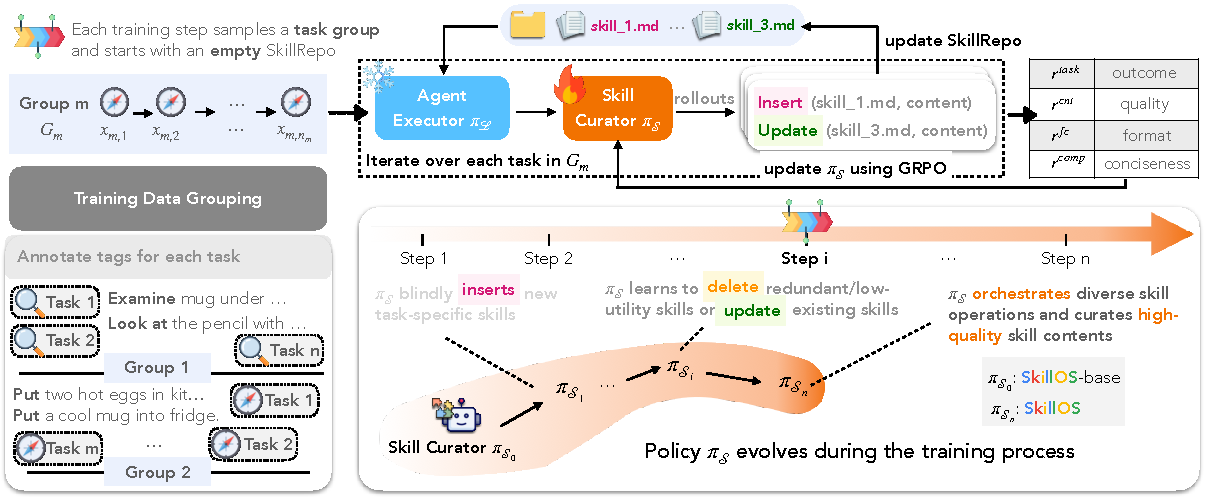
\includegraphics[width=0.98\textwidth]{figures/SkillOS.pdf}
\end{center}
\vspace{-3mm}
\caption{\ours{} training pipeline. Each training step samples a group of related tasks and initializes an empty \textsc{SkillRepo}. $\pi_{\mathcal{S}}$ is optimized with composite rewards, enabling self-evolution.
}
\label{fig: skillagent}
\vspace{-5mm}
\end{figure}

\subsubsection{Training Instance Construction}\label{sec:training_instance_construction}

To provide downstream learning signals for skill curation, we construct each training instance as a group of related tasks that are solved sequentially. Within each group, \textsc{SkillRepo} is updated by the curator $\pi_{\mathcal{s}}$ after each task, allowing skills derived from earlier experiences to be evaluated by whether they help solve related future tasks.
This also differs from prior work that focuses on short-horizon transfer~\citep{DBLP:journals/corr/abs-2512-17102, DBLP:journals/corr/abs-2602-10652}, where our grouped formulation exposes the curator to longer skill-evolution trajectories and provides denser feedback for learning complex curation operations.  

Concretely, for each task $x_i$ in $\mathcal{D}=\{x_i\}_{i=1}^{N}$, we first annotate each instance with a set of skill-relevant attributes. Formally, for each $x_i$, we use Gemini-2.5-Pro~\citep{DBLP:journals/corr/abs-2507-06261} to produce a set of tags:
\vspace{-1mm}
\[
Z_i = \{z_i^{1}, z_i^{2}, \dots, z_i^{|Z_i|}\},
\]
where each attribute $z_i$ captures a salient aspect of the task $x_i$, such as topic and common pitfalls. For example, in mathematical reasoning, attributes may include labels such as ``algebra'' or ``Fourier transformation''. These attributes serve as proxies for task-relatedness and potential skill dependency.

Based on the annotated attributes, we then partition $\mathcal{D}$ into a collection of $M$ task groups using the similarity of attributes of these data samples:
\vspace{-1mm}
\[
\mathcal{D}=\{G_1, G_2, \dots, G_{M}\}, \qquad G_m = \{x_{m,1}, x_{m,2}, \dots, x_{m,|G_m|}\},
\]
where all instances within the same group $G_m$ exhibit non-trivial dependency in terms of required skills. Detailed description of data processing and grouping algorithms can be found in Appendix~\ref{app:group_training}.


\subsubsection{Training Loop and Policy Optimization}\label{sec:reward_design} 

We employ Grouped Reward Policy Optimization (GRPO~\cite{DBLP:journals/corr/abs-2402-03300}) for its training stability and sample efficiency. The training loop shown in Algorithm~\ref{alg:mem_grpo} optimizes the skill curator policy $\pi_{\mathcal{S}}$ to maximize a composite reward function over the distribution of generated traces. 
% The reward for the skill curator's curations $c_{b}$ for the $b$-th batch within one training step combines four signals:
For a task group $G=(x_1,\dots,x_{|G|})$, the curator produces a sequence of curation decisions
$c=(c_1,\dots,c_{|G|})$ as the executor proceeds through the group. Each training step, the reward combines four signals:
\setlength{\abovedisplayskip}{0pt}
\setlength{\belowdisplayskip}{0pt}
\setlength{\abovedisplayshortskip}{0pt}
\setlength{\belowdisplayshortskip}{0pt}
\begin{equation}
    r \;=\; \underbrace{r^{\text{task}}}_{\text{task outcome}}
    + \;\lambda_{\mathrm{f}} \underbrace{r^{\text{fc}}}_{\text{function call}}
    + \;\lambda_{\mathrm{u}} \underbrace{r^{\text{cnt}}}_{\text{content quality}}
    + \;\lambda_{\mathrm{c}} \underbrace{r^{\text{comp}}}_{\text{compression}}
    \label{eq:reward}
\end{equation}

\noindent\textbf{Task outcome reward.}\;
The first task uses an empty \textsc{SkillRepo}, before any curator update occurs.
We thus define the task outcome reward as the average success over the remaining tasks as $r^{\text{task}}
    =
    \frac{1}{|G|-1}
    \sum_{i=2}^{|G|}
    \mathbbm{1}(\xi_i)$,
which provides executor-grounded signal on downstream performance achieved by the evolving \textsc{SkillRepo} from $\pi_{\mathcal{S}}$.

\noindent\textbf{Function call reward.}\;
The function call reward measures whether the curator produces valid skill operations. 
For each curation decision $c_i$, let $\mathrm{Valid}(c_i)$ be the fraction of generated function calls that are valid and successfully executed.
We define the function call reward as $r^{\text{fc}}
    =
    \frac{1}{|G|}
    \sum_{i=1}^{|G|}
    \mathrm{Valid}(c_i)$.


\begin{algorithm}[t]
\caption{Training Skill Curator with Task Groups using GRPO}
\label{alg:mem_grpo}
\begin{algorithmic}[1]
\For{each training step}
    \State $G=(x_1,\dots,x_{|G|})$,\ $\mathcal{S}\leftarrow \emptyset$
        \Comment{\textcolor{googleblue}{\textit{Sample a task group and initialize SkillRepo}}}
    \For{task index $i = 1,\dots,|G|$}
        \State $\tilde{\mathcal{S}} \leftarrow \textsc{BM25}\!\left(x_i,\; \mathcal{S}\right)$
            \Comment{\textcolor{googleblue}{\textit{Retrieve relevant skills}}}
        \State $\xi_{i} \leftarrow \textsc{RunTask}\!\left(\tilde{\mathcal{S}},\;\pi_{\mathcal{L}},\;x_i\right)$
            \Comment{\textcolor{googleblue}{\textit{Run inference on frozen executor}}}
        \State $c_{i} \sim \pi_{\mathcal{S}}\!\left(\cdot \;\middle|\; \xi_i, \tilde{\mathcal{S}}\right)$
            \Comment{\textcolor{googleblue}{\textit{Sample a rollout from skill curator}}}
        \State $\mathcal{S} \leftarrow \textsc{ApplyOps}\!\left(\mathcal{S},\; c_{i}\right)$
            \Comment{\textcolor{googleblue}{\textit{Apply \texttt{insert}/\texttt{update}/\texttt{delete}}}}
    \EndFor
    \State $r \leftarrow \textsc{CalculateReward}(\xi, c)$
    \State $\textsc{Update}\ \pi_{\mathcal{S}}$
        \Comment{\textcolor{googleblue}{\textit{Update skill curator using GRPO}}}
\EndFor
\end{algorithmic}
\end{algorithm}


\noindent\textbf{Compression reward.}\;
To discourage verbatim trajectory copying, we reward concise repository updates. 
Let $\mathcal{S}_i$ denote the skill repository after applying $c_i$, and let $\chi_i$ denote the curator input context at position $i$.
We define $r^{\text{comp}}
    =
    \frac{1}{|G|}
    \sum_{i=1}^{|G|}
    \left(
    1 - \frac{|\mathcal{S}_i|}{|\chi_i|}
    \right)$,
where $|\mathcal{S}_i|$ and $|\chi_i|$ denote token lengths.
This encourages the curator to distill reusable skills rather than store raw trajectories.


\noindent\textbf{Content quality reward.}\;
The content quality reward evaluates whether the curated skills are semantically meaningful and likely to be useful for future tasks. 
Let $\mathrm{Judge}(c_i)$ denote the scalar score assigned by an external judge (Qwen3-32B) $c_i$, we compute the reward as $
    r^{\text{cnt}}
    =
    \frac{1}{|G|}
    \sum_{i=1}^{|G|}
    \mathrm{Judge}(c_i)$.

For each task group $G$, we sample $N$ independent rollouts of the \emph{entire curation sequence} from $\pi_{\mathcal{S}}$. Within each rollout, the executor produces trajectory $\xi_i$ using the skill repository $\mathcal{S}^{i}$ resulting from previous curations $c_{<i}$ till task position $i$ with the same training task group, so different rollouts evolve different repository histories. The GRPO advantage is computed as:
$     A^{n} = r^{n} - \frac{1}{N}\sum_{n'=1}^{N} r^{n'},$
where $r^{n}$ is the composite reward (Eq.~\ref{eq:reward}) for the $n$-th rollout.
We optimize $\pi_{\mathcal{S}}$ with a clipped surrogate objective over all curation steps $i = 1, \ldots, |G|$:
\begin{equation}
    \mathcal{L} = \mathbb{E}_{n} \!\left[\min\!\left(\rho^{n}\,A^{n},\; \mathrm{clip}\!\left(\rho^{n},\, 1{-}\epsilon,\, 1{+}\epsilon\right)\!A^{n}\right)\right]
    \label{eq:grpo}
\end{equation}
where $\rho^{n} = \pi_{\mathcal{S}}(c^{n} \mid \chi) \,/\, \pi_{\theta_{old}}(c^{n} \mid \chi)$ is the importance ratio. The advantage $A^{n}$ is assigned uniformly to all tokens in $c^{n}$, and we discard the KL term in GRPO to encourage policy exploration.
